\documentclass{article} 

\usepackage{minted} % This package allows to highlight the syntax of codes.
\usepackage{geometry} % This package allows the editing of the page layout
\usepackage{amsmath}  % This package allows the use of a large range of mathematical formula, commands, and symbols
\usepackage{graphicx}  % This package allows the importing of images
\usepackage{hyperref} % This package allows hyperlink reference. The context here is to create hyperlink in table of contents.
\hypersetup{
    colorlinks,
    citecolor=black,
    filecolor=black,
    linkcolor=black,
    urlcolor=black
}
\graphicspath{ {./figures/} }

\begin{document}

\begin{titlepage}
\centering % Centre everything on the title page

\scshape % Use small caps for all text on the title page

\vspace*{\baselineskip} % White space at the top of the page

\rule{\textwidth}{1.6pt}\vspace*{-\baselineskip}\vspace*{2pt} % Thick horizontal rule
\rule{\textwidth}{0.4pt} % Thin horizontal rule

\vspace{0.75\baselineskip} % Whitespace above the title

{\LARGE OBJECT ORIENTED \\ \vspace{0.75\baselineskip}SOFTWARE DEVELOPMENT} % Title

\vspace{0.75\baselineskip} % Whitespace below the title

\rule{\textwidth}{0.4pt}\vspace*{-\baselineskip}\vspace{3.2pt} % Thin horizontal rule
\rule{\textwidth}{1.6pt} % Thick horizontal rule

\vfill

{\LARGE LAB II }

\vspace{0.5\baselineskip} 

{\scshape\Large Title : Implementation of Creation Design Patterns \\} 

\vfill

By

\vspace{0.5\baselineskip} 

{\scshape\Large Arjun Prasad Adhikari \\} 
\vspace{0.5\baselineskip} % 

\textit{Sixth Semster} % Your semester
\vspace{0.5\baselineskip}

\textit{Roll No. 6} % Your roll no
\vfill % Whitespace 

\textit{Gandaki College of Engineering and Science} 
\vspace{1\baselineskip}

Dec 11 2020 % Publication year


\end{titlepage}
\newpage
\tableofcontents
\newpage
\listoffigures
\newpage

\section{Adapter Pattern}

Adapter pattern works as a bridge between two incompatible interfaces. This type of design pattern comes under structural pattern as this pattern combines the capability of two independent interfaces.

This pattern involves a single class which is responsible to join functionalities of independent or incompatible interfaces. A real life example could be a case of card reader which acts as an adapter between memory card and a laptop. You plugin the memory card into card reader and card reader into the laptop so that memory card can be read via laptop.

We are demonstrating use of Adapter pattern via following example in which an audio player device can play mp3 files only and wants to use an advanced audio player capable of playing vlc and mp4 files. 

\subsection{Implementation}

We have a MediaPlayer interface and a concrete class AudioPlayer implementing the MediaPlayer interface. AudioPlayer can play mp3 format audio files by default.

We are having another interface AdvancedMediaPlayer and concrete classes implementing the AdvancedMediaPlayer interface. These classes can play vlc and mp4 format files.

We want to make AudioPlayer to play other formats as well. To attain this, we have created an adapter class MediaAdapter which implements the MediaPlayer interface and uses AdvancedMediaPlayer objects to play the required format.

AudioPlayer uses the adapter class MediaAdapter passing it the desired audio type without knowing the actual class which can play the desired format. AdapterPatternDemo, our demo class will use AudioPlayer class to play various formats.

\subsection{Class Diagram}

\begin{figure}[h]
\centering
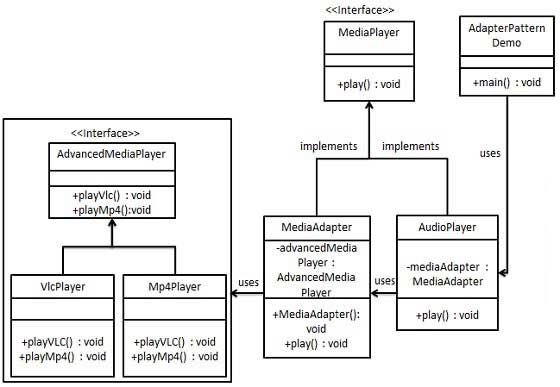
\includegraphics[scale=0.7]{adapter}
\caption{Class Diagram of Adapter Pattern}
\end{figure}

\newpage
\subsection{Source Code (Java)}

\subsubsection{MediaPlayer Interface}

\begin{minted}{java}
public interface MediaPlayer {
   public void play(String audioType, String fileName);
}
\end{minted}

\subsubsection{AdvancedMediaPlayer Interface}

\begin{minted}{java}
public interface AdvancedMediaPlayer {	
   public void playVlc(String fileName);
   public void playMp4(String fileName);
}
\end{minted}

\subsubsection{AdvancedMediaPlayer Class}

\begin{minted}{java}
public class VlcPlayer implements AdvancedMediaPlayer{
   @Override
   public void playVlc(String fileName) {
      System.out.println("Playing vlc file. Name: "+ fileName);		
   }

   @Override
   public void playMp4(String fileName) {
      //do nothing
   }
}
\end{minted}

\subsubsection{Mp4Player Class}

\begin{minted}{java}
public class Mp4Player implements AdvancedMediaPlayer{

   @Override
   public void playVlc(String fileName) {
      //do nothing
   }

   @Override
   public void playMp4(String fileName) {
      System.out.println("Playing mp4 file. Name: "+ fileName);		
   }
}
\end{minted}

\subsubsection{MediaAdapter Class}

\begin{minted}{java}
public class MediaAdapter implements MediaPlayer {

   AdvancedMediaPlayer advancedMusicPlayer;

   public MediaAdapter(String audioType){
   
      if(audioType.equalsIgnoreCase("vlc") ){
         advancedMusicPlayer = new VlcPlayer();			
         
      }else if (audioType.equalsIgnoreCase("mp4")){
         advancedMusicPlayer = new Mp4Player();
      }	
   }

   @Override
   public void play(String audioType, String fileName) {
   
      if(audioType.equalsIgnoreCase("vlc")){
         advancedMusicPlayer.playVlc(fileName);
      }
      else if(audioType.equalsIgnoreCase("mp4")){
         advancedMusicPlayer.playMp4(fileName);
      }
   }
}
\end{minted}

\subsubsection{AudioPlayer Class}

\begin{minted}{java}
public class AudioPlayer implements MediaPlayer {
   MediaAdapter mediaAdapter; 

   @Override
   public void play(String audioType, String fileName) {		

      //inbuilt support to play mp3 music files
      if(audioType.equalsIgnoreCase("mp3")){
         System.out.println("Playing mp3 file. Name: " + fileName);			
      } 
      
      //mediaAdapter is providing support to play other file formats
      else if(audioType.equalsIgnoreCase("vlc") || audioType.equalsIgnoreCase("mp4")){
         mediaAdapter = new MediaAdapter(audioType);
         mediaAdapter.play(audioType, fileName);
      }
      
      else{
         System.out.println("Invalid media. " + audioType + " format not supported");
      }
   }   
}
\end{minted}

\subsubsection{Driver Class}

\begin{minted}{java}
public class AdapterPatternDemo {
   public static void main(String[] args) {
      AudioPlayer audioPlayer = new AudioPlayer();

      audioPlayer.play("mp3", "beyond the horizon.mp3");
      audioPlayer.play("mp4", "alone.mp4");
      audioPlayer.play("vlc", "far far away.vlc");
      audioPlayer.play("avi", "mind me.avi");
   }
}
\end{minted}

\subsection{Output}

\begin{minted}{text}
Playing mp3 file. Name: beyond the horizon.mp3
Playing mp4 file. Name: alone.mp4
Playing vlc file. Name: far far away.vlc
Invalid media. avi format not supported
\end{minted}

\newpage
\section{Bridge Pattern}

Bridge is used when we need to decouple an abstraction from its implementation so that the two can vary independently. This type of design pattern comes under structural pattern as this pattern decouples implementation class and abstract class by providing a bridge structure between them.

This pattern involves an interface which acts as a bridge which makes the functionality of concrete classes independent from interface implementer classes. Both types of classes can be altered structurally without affecting each other.

We are demonstrating use of Bridge pattern via following example in which a circle can be drawn in different colors using same abstract class method but different bridge implementer classes. 

\subsection{Implementation}

We have a DrawAPI interface which is acting as a bridge implementer and concrete classes RedCircle, GreenCircle implementing the DrawAPI interface. Shape is an abstract class and will use object of DrawAPI. BridgePatternDemo, our demo class will use Shape class to draw different colored circle.

\subsection{Class Diagram}

\begin{figure}[h]
\centering
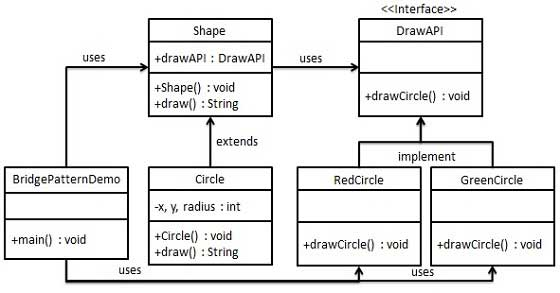
\includegraphics[scale=0.7]{bridge}
\caption{Class Diagram of Bridge Pattern}
\end{figure}

\newpage
\subsection{Source Code (Java)}

\subsubsection{DrawAPI Interface}

\begin{minted}{java}
public interface DrawAPI {
   public void drawCircle(int radius, int x, int y);
}
\end{minted}

\subsubsection{RedCircle Class}

\begin{minted}{java}
public class RedCircle implements DrawAPI {
   @Override
   public void drawCircle(int radius, int x, int y) {
      System.out.println(
		"Drawing Circle[ color: red, radius: " + radius + ", x: " + x + ", " + y + "]"
	);
   }
}
\end{minted}

\subsubsection{GreenCircle Class}

\begin{minted}{java}
public class GreenCircle implements DrawAPI {
   @Override
   public void drawCircle(int radius, int x, int y) {
      System.out.println(
		"Drawing Circle[ color: green, radius: " + radius + ", x: " + x + ", " + y + "]"
	);
   }
}
\end{minted}

\subsubsection{Shape abstract Class}

\begin{minted}{java}
public abstract class Shape {
   protected DrawAPI drawAPI;
   
   protected Shape(DrawAPI drawAPI){
      this.drawAPI = drawAPI;
   }
   public abstract void draw();	
}
\end{minted}

\subsubsection{Circle Class}

\begin{minted}{java}
public class Circle extends Shape {
   private int x, y, radius;

   public Circle(int x, int y, int radius, DrawAPI drawAPI) {
      super(drawAPI);
      this.x = x;  
      this.y = y;  
      this.radius = radius;
   }

   public void draw() {
      drawAPI.drawCircle(radius,x,y);
   }
}
\end{minted}

\subsubsection{Driver Class}

\begin{minted}{java}
public class BridgePatternDemo {
   public static void main(String[] args) {
      Shape redCircle = new Circle(100,100, 10, new RedCircle());
      Shape greenCircle = new Circle(100,100, 10, new GreenCircle());

      redCircle.draw();
      greenCircle.draw();
   }
}
\end{minted}

\subsection{Output}

\begin{minted}{text}
Drawing Circle[ color: red, radius: 10, x: 100, 100]
Drawing Circle[  color: green, radius: 10, x: 100, 100]
\end{minted}

\newpage
\section{Composite Pattern}

Composite pattern is used where we need to treat a group of objects in similar way as a single object. Composite pattern composes objects in term of a tree structure to represent part as well as whole hierarchy. This type of design pattern comes under structural pattern as this pattern creates a tree structure of group of objects.

This pattern creates a class that contains group of its own objects. This class provides ways to modify its group of same objects.

We are demonstrating use of composite pattern via following example in which we will show employees hierarchy of an organization.

\subsection{Implementation}

We have a class Employee which acts as composite pattern actor class. CompositePatternDemo, our demo class will use Employee class to add department level hierarchy and print all employees.

\subsection{Class Diagram}

\begin{figure}[h]
\centering
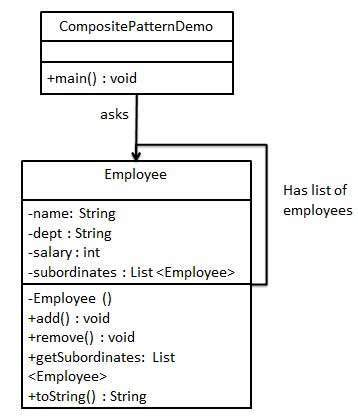
\includegraphics[scale=0.5]{composite}
\caption{Class Diagram of Composite Pattern}
\end{figure}

\newpage
\subsection{Source Code (Java)}

\subsubsection{Employee Class}

\begin{minted}{java}
import java.util.ArrayList;
import java.util.List;

public class Employee {
   private String name;
   private String dept;
   private int salary;
   private List<Employee> subordinates;

   // constructor
   public Employee(String name,String dept, int sal) {
      this.name = name;
      this.dept = dept;
      this.salary = sal;
      subordinates = new ArrayList<Employee>();
   }

   public void add(Employee e) {
      subordinates.add(e);
   }

   public void remove(Employee e) {
      subordinates.remove(e);
   }

   public List<Employee> getSubordinates(){
     return subordinates;
   }

   public String toString(){
      return ("Employee :[ Name : " + name + ", dept : " + dept + ", salary :" + salary+" ]");
   }   
}
\end{minted}

\subsubsection{Driver Class}

\begin{minted}{java}
public class CompositePatternDemo {
   public static void main(String[] args) {
   
      Employee CEO = new Employee("John","CEO", 30000);

      Employee headSales = new Employee("Robert","Head Sales", 20000);

      Employee headMarketing = new Employee("Michel","Head Marketing", 20000);

      Employee clerk1 = new Employee("Laura","Marketing", 10000);
      Employee clerk2 = new Employee("Bob","Marketing", 10000);

      Employee salesExecutive1 = new Employee("Richard","Sales", 10000);
      Employee salesExecutive2 = new Employee("Rob","Sales", 10000);

      CEO.add(headSales);
      CEO.add(headMarketing);

      headSales.add(salesExecutive1);
      headSales.add(salesExecutive2);

      headMarketing.add(clerk1);
      headMarketing.add(clerk2);

      //print all employees of the organization
      System.out.println(CEO); 
      
      for (Employee headEmployee : CEO.getSubordinates()) {
         System.out.println(headEmployee);
         
         for (Employee employee : headEmployee.getSubordinates()) {
            System.out.println(employee);
         }
      }		
   }
}
\end{minted}

\subsection{Output}

\begin{minted}{text}
Employee :[ Name : John, dept : CEO, salary :30000 ]
Employee :[ Name : Robert, dept : Head Sales, salary :20000 ]
Employee :[ Name : Richard, dept : Sales, salary :10000 ]
Employee :[ Name : Rob, dept : Sales, salary :10000 ]
Employee :[ Name : Michel, dept : Head Marketing, salary :20000 ]
Employee :[ Name : Laura, dept : Marketing, salary :10000 ]
Employee :[ Name : Bob, dept : Marketing, salary :10000 ]
\end{minted}

\newpage
\section{Decorator Pattern}

Decorator pattern allows a user to add new functionality to an existing object without altering its structure. This type of design pattern comes under structural pattern as this pattern acts as a wrapper to existing class.

This pattern creates a decorator class which wraps the original class and provides additional functionality keeping class methods signature intact.

We are demonstrating the use of decorator pattern via following example in which we will decorate a shape with some color without alter shape class.

\subsection{Implementation}

We're going to create a Shape interface and concrete classes implementing the Shape interface. We will then create an abstract decorator class ShapeDecorator implementing the Shape interface and having Shape object as its instance variable.

RedShapeDecorator is concrete class implementing ShapeDecorator.

DecoratorPatternDemo, our demo class will use RedShapeDecorator to decorate Shape objects.

\subsection{Class Diagram}

\begin{figure}[h]
\centering
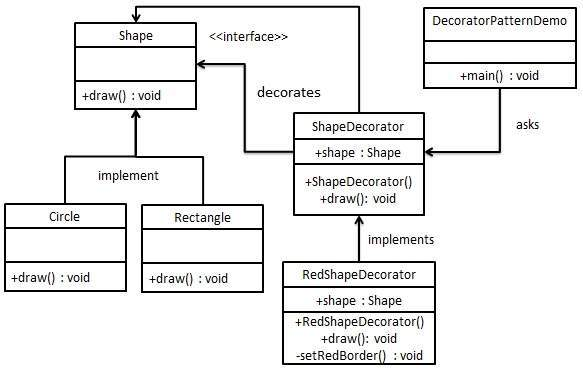
\includegraphics[scale=0.5]{decorator}
\caption{Class Diagram of Decorator Pattern}
\end{figure}

\newpage
\subsection{Source Code (Java)}

\subsubsection{Shape Interface}

\begin{minted}{java}
public interface Shape {
   void draw();
}
\end{minted}

\subsubsection{Rectangle Class}

\begin{minted}{java}
public class Rectangle implements Shape {

   @Override
   public void draw() {
      System.out.println("Shape: Rectangle");
   }
}
\end{minted}

\subsubsection{Circle Class}

\begin{minted}{java}
public class Circle implements Shape {

   @Override
   public void draw() {
      System.out.println("Shape: Circle");
   }
}
\end{minted}

\subsubsection{ShapeDecorator abstract Class}

\begin{minted}{java}
public abstract class ShapeDecorator implements Shape {
   protected Shape decoratedShape;

   public ShapeDecorator(Shape decoratedShape){
      this.decoratedShape = decoratedShape;
   }

   public void draw(){
      decoratedShape.draw();
   }	
}
\end{minted}

\subsubsection{RedShapeDecorator Class}

\begin{minted}{java}
public class RedShapeDecorator extends ShapeDecorator {

   public RedShapeDecorator(Shape decoratedShape) {
      super(decoratedShape);		
   }

   @Override
   public void draw() {
      decoratedShape.draw();	       
      setRedBorder(decoratedShape);
   }

   private void setRedBorder(Shape decoratedShape){
      System.out.println("Border Color: Red");
   }
}
\end{minted}

\subsubsection{Driver Class}

\begin{minted}{java}
public class DecoratorPatternDemo {
   public static void main(String[] args) {

      Shape circle = new Circle();

      Shape redCircle = new RedShapeDecorator(new Circle());

      Shape redRectangle = new RedShapeDecorator(new Rectangle());
      System.out.println("Circle with normal border");
      circle.draw();

      System.out.println("\nCircle of red border");
      redCircle.draw();

      System.out.println("\nRectangle of red border");
      redRectangle.draw();
   }
}
\end{minted}

\subsection{Output}

\begin{minted}{text}
Circle with normal border
Shape: Circle

Circle of red border
Shape: Circle
Border Color: Red

Rectangle of red border
Shape: Rectangle
Border Color: Red
\end{minted}

\newpage
\section{Facade Pattern}

Facade pattern hides the complexities of the system and provides an interface to the client using which the client can access the system. This type of design pattern comes under structural pattern as this pattern adds an interface to existing system to hide its complexities.

This pattern involves a single class which provides simplified methods required by client and delegates calls to methods of existing system classes.

\subsection{Implementation}

We are going to create a Shape interface and concrete classes implementing the Shape interface. A facade class ShapeMaker is defined as a next step.

ShapeMaker class uses the concrete classes to delegate user calls to these classes. FacadePatternDemo, our demo class, will use ShapeMaker class to show the results.

\subsection{Class Diagram}

\begin{figure}[h]
\centering
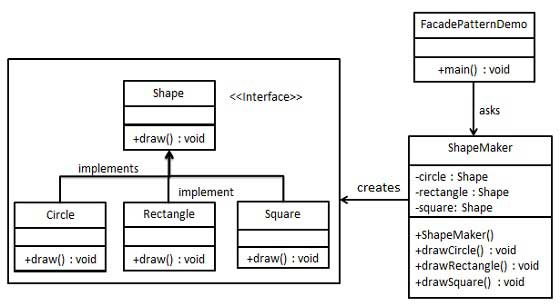
\includegraphics[scale=0.7]{facade}
\caption{Class Diagram of Facade Pattern}
\end{figure}

\newpage
\subsection{Source Code (Java)}

\subsubsection{Shape Interface}

\begin{minted}{java}
public interface Shape {
   void draw();
}
\end{minted}

\subsubsection{Rectangle Class}

\begin{minted}{java}
public class Rectangle implements Shape {

   @Override
   public void draw() {
      System.out.println("Rectangle::draw()");
   }
}
\end{minted}

\subsubsection{Square Class}

\begin{minted}{java}
public class Square implements Shape {

   @Override
   public void draw() {
      System.out.println("Square::draw()");
   }
}
\end{minted}

\subsubsection{Circle Class}

\begin{minted}{java}
public class Circle implements Shape {

   @Override
   public void draw() {
      System.out.println("Circle::draw()");
   }
}
\end{minted}

\subsubsection{ShapeMaker Class}

\begin{minted}{java}
public class ShapeMaker {
   private Shape circle;
   private Shape rectangle;
   private Shape square;

   public ShapeMaker() {
      circle = new Circle();
      rectangle = new Rectangle();
      square = new Square();
   }

   public void drawCircle(){
      circle.draw();
   }
   public void drawRectangle(){
      rectangle.draw();
   }
   public void drawSquare(){
      square.draw();
   }
}
\end{minted}

\subsubsection{Driver Class}

\begin{minted}{java}
public class FacadePatternDemo {
   public static void main(String[] args) {
      ShapeMaker shapeMaker = new ShapeMaker();

      shapeMaker.drawCircle();
      shapeMaker.drawRectangle();
      shapeMaker.drawSquare();		
   }
}
\end{minted}

\subsection{Output}

\begin{minted}{text}
Circle::draw()
Rectangle::draw()
Square::draw()
\end{minted}

\newpage
\section{Proxy Pattern}

In proxy pattern, a class represents functionality of another class. This type of design pattern comes under structural pattern.

In proxy pattern, we create object having original object to interface its functionality to outer world.

\subsection{Implementation}

We are going to create an Image interface and concrete classes implementing the Image interface. ProxyImage is a a proxy class to reduce memory footprint of RealImage object loading.

ProxyPatternDemo, our demo class, will use ProxyImage to get an Image object to load and display as it needs.

\subsection{Class Diagram}

\begin{figure}[h]
\centering
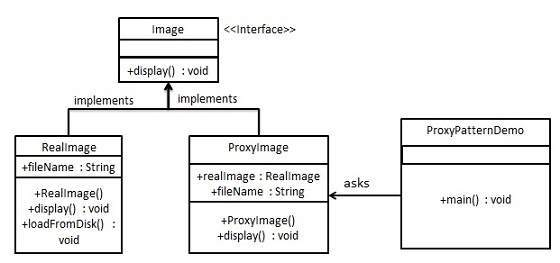
\includegraphics[scale=0.7]{proxy}
\caption{Class Diagram of Proxy Pattern}
\end{figure}

\newpage
\subsection{Source Code (Java)}

\subsubsection{Image Interface}

\begin{minted}{java}
public interface Image {
   void display();
}
\end{minted}

\subsubsection{RealImage Class}

\begin{minted}{java}
public class RealImage implements Image {

   private String fileName;

   public RealImage(String fileName){
      this.fileName = fileName;
      loadFromDisk(fileName);
   }

   @Override
   public void display() {
      System.out.println("Displaying " + fileName);
   }

   private void loadFromDisk(String fileName){
      System.out.println("Loading " + fileName);
   }
}
\end{minted}

\subsubsection{ProxyImage Class}

\begin{minted}{java}
public class ProxyImage implements Image{

   private RealImage realImage;
   private String fileName;

   public ProxyImage(String fileName){
      this.fileName = fileName;
   }

   @Override
   public void display() {
      if(realImage == null){
         realImage = new RealImage(fileName);
      }
      realImage.display();
   }
}
\end{minted}

\subsubsection{Driver Class}

\begin{minted}{java}
public class ProxyPatternDemo {
	
   public static void main(String[] args) {
      Image image = new ProxyImage("test_10mb.jpg");

      //image will be loaded from disk
      image.display(); 
      System.out.println("");
      
      //image will not be loaded from disk
      image.display(); 	
   }
}
\end{minted}

\subsection{Output}

\begin{minted}{text}
Loading test_10mb.jpg
Displaying test_10mb.jpg

Displaying test_10mb.jpg
\end{minted}


\end{document}